\section{Projekt robota}
\subsection{Założenia projektowe}
Wykonany robot powinien być jak najmniejszy i najprostszy w wykonaniu oraz sterowaniu tak aby móc przetestować przy jego pomocy działanie algorytmu A*. 
Robot będzie zbudowany z platformy, do której zostaną przyczepione napędy, elektronika sterująca oraz bateria. 
Do platformy zostaną przymocowane dwa gotowe moduły napędowe składające się z silnika, przekładni oraz dużego koła. 
Aby pojazd stał stabilnie, doczepione zostanie trzecie koło obracające się swobodnie w każdym kierunku.
Całość będzie sterowana przy pomocy mikroprocesora ESP32 oraz dwukanałowego sterownika silników DC opartym na układzie L298n.
Za zasilanie będzie odpowiadał litowo-jonowy akumulator 4S.

\subsection{Projektowanie robota w środowisku CAD}
Podstawa robota utrzymująca wszystkie komponenty zostanie wydrukowana na drukarce 3D, a
model platformy i pozostałych posiadanych elementów został wykonany w programie Fusion 360.
Wykonane modele modułów napędowych, przedniego kółka oraz baterii pozwoliły na optymalne rozmieszczenie wszystkich elementów.

\begin{figure}[H]
	\centering
	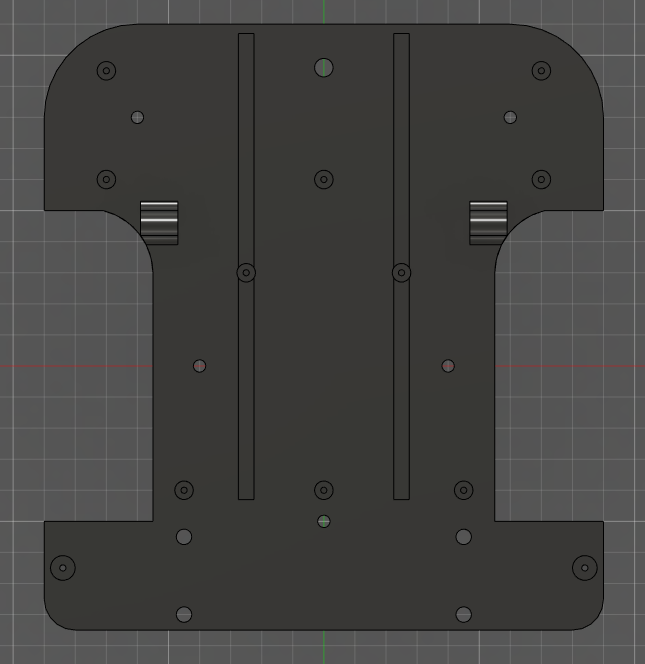
\includegraphics[width=8cm]{pages/robot/zdjecia/robotModelRama.png}
	\caption{Widok z góry na podwozie robota}
	\label{Fig:robotModelRama}
\end{figure}

Model został przygotowany w programie Ultimaker Cura i wydrukowane z filamentu PLA.
Temperatur głowicy wynosiła 220$ ^\circ C$ a stołu 60$ ^\circ C$. Aby przyśpieszyć wydruk wysokość warstwy została ustawiona na 0,2mm. 
Żeby zwiększyć wytrzymałość i lepiej zgrzać warstwy, temperatura głowicy została lekko zawyżona względem wymagań producenta filamentu,
a model posiada dwa dodatkowe wsporniki wzdłuż platformy.

\begin{figure}[H]
	\centering
	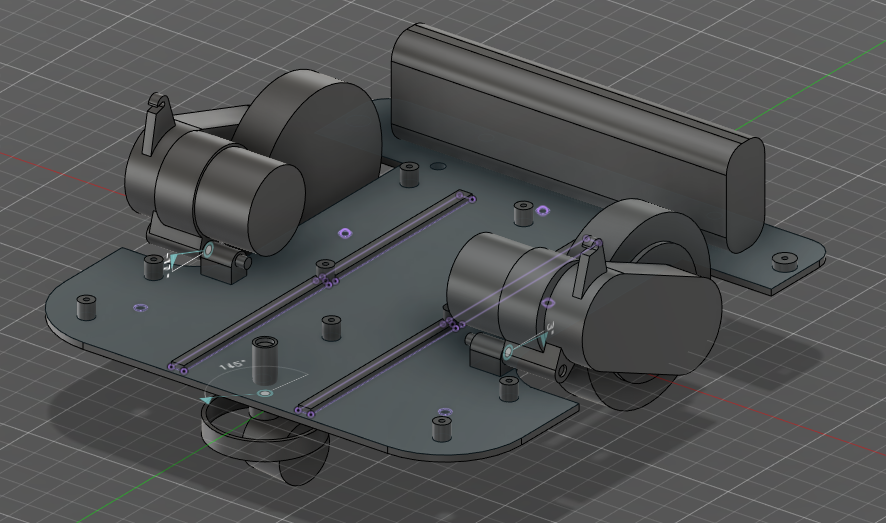
\includegraphics[width=14cm]{pages/robot/zdjecia/robotModelCaly.png}
	\caption{Model robota z modułami}
	\label{fig:robotModelCaly}
\end{figure}

Na powyższym zdjęciu widać zaprojektowaną ramę wraz z odpowiednio ustawionymi gotowymi modułami. 
Moduły napędowe zaczepione są przy pomocy fabrycznego trzpienia wciskanego w ramę. 
Takie rozwiązanie oznacza że napęd może obracać się w wokół własnej osi. Aby zapewnić stały i równomierny docisk koła do podłoża,
napęd został połączony sprężyną z ramą. 

\subsection{Elektronika sterująca robotem}
Do bezprzewodowego sterowania robotem zostanie wykorzystany moduł ESP32, dla którego zostanie przygotowana odpowiednia płytka 
z wyprowadzeniami do enkoderów silnika oraz ich sterownika. Schemat i projekt płytki drukowanej został wykonany w programie KiCad. 
\begin{figure}[H]
	\centering
	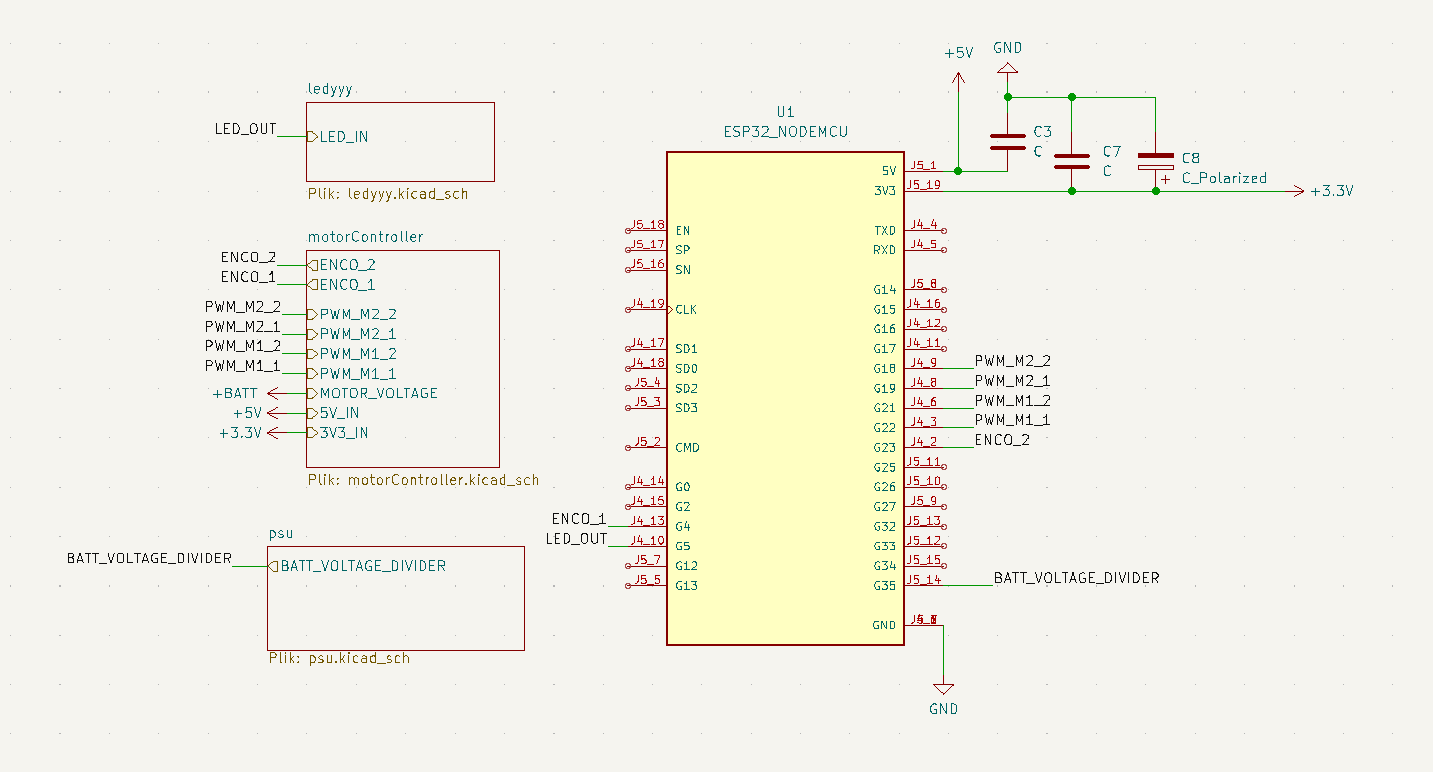
\includegraphics[width=18cm]{pages/robot/zdjecia/kicad/schematCaly.png}
	\caption{Schemat połączeń pomiędzy modułami}
	\label{Fig:schematKiCad}
\end{figure}

Przedstawiony powyżej schemat został podzielony na kilka sekcji. 
Najbardziej rozbudowana jest sekcja zasilania, która poprzez dwa stabilizatory liniowe obniża napięcie z 16,8V do 5V. Mikroprocesor zasilany jest
napięciem 3,3V przygotowanym przez układ wlutowany na płytce deweloperskiej. Każda linia zasilania filtrowana jest przez kondensator elektrolityczny 
i ceramiczny, wynika to z dużego poboru prądu podczas komunikacji z WiFi. 

Kolejny segment zawiera po dwa złącza na silnik. Jedno złącze służy do połączenia z silnikiem, zasilania i odbierania danych z enkodera.
Drugie złącze służy do połączenia sterownika z silnikiem i dwoma kanałami PWM, pozwalającymi na płynne sterowanie kierunkiem i prędkością obrotową silnika.

Trzeci segment zawiera świecące diody programowalne służące do sygnalizacji stanu robota. Zaletą wykorzystanych tych diod jest szeregowe połączenie 
i bezpośrednie zasilanie z lini 5V. Ostatnia podłączona dioda jest na stałe i sygnalizuje podłączoną baterię.

Ostatnia sekcja to połączenia pomiędzy modułem deweloperskim ESP32 a resztą układu. Mikroprocesor pracuje w logice 3,3V a sterownik silników 5V. 
Mimo tego, nie są potrzebne żadne układy zamieniające poziomy napięć. 
Dodatkowo obok wyprowadzeń modułu widać dodatkowe kondensatory filtrujące zasilanie. 
 
Użyte moduły napędowe posiadają enkoder inkrementalny zbudowany z czujnika halla i tarczy magnetycznej zamocowanej na wale silnika.
Silniki sterowane są modułem z układem L298n, a prędkość ustalana jest poprzez odpowiednio generowany sygnał PWM.
\begin{figure}[H]
	\centering
	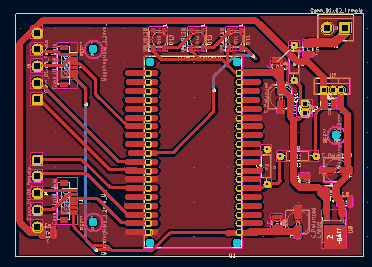
\includegraphics[width=10cm]{pages/robot/zdjecia/kicad/kiCad_PCB.png}
	\caption{Projekt PCB}
	\label{Fig:kiCadPCB}
\end{figure}

Na widocznym powyżej zdjęciu widać ostateczną wersje płytki drukowanej. Większość połączeń na płytce zrealizowana jest poprzez górną warstwę miedzi,
jednak widać kilka ścieżek w dolnej warstwie.

\begin{figure}[H]
	\centering
	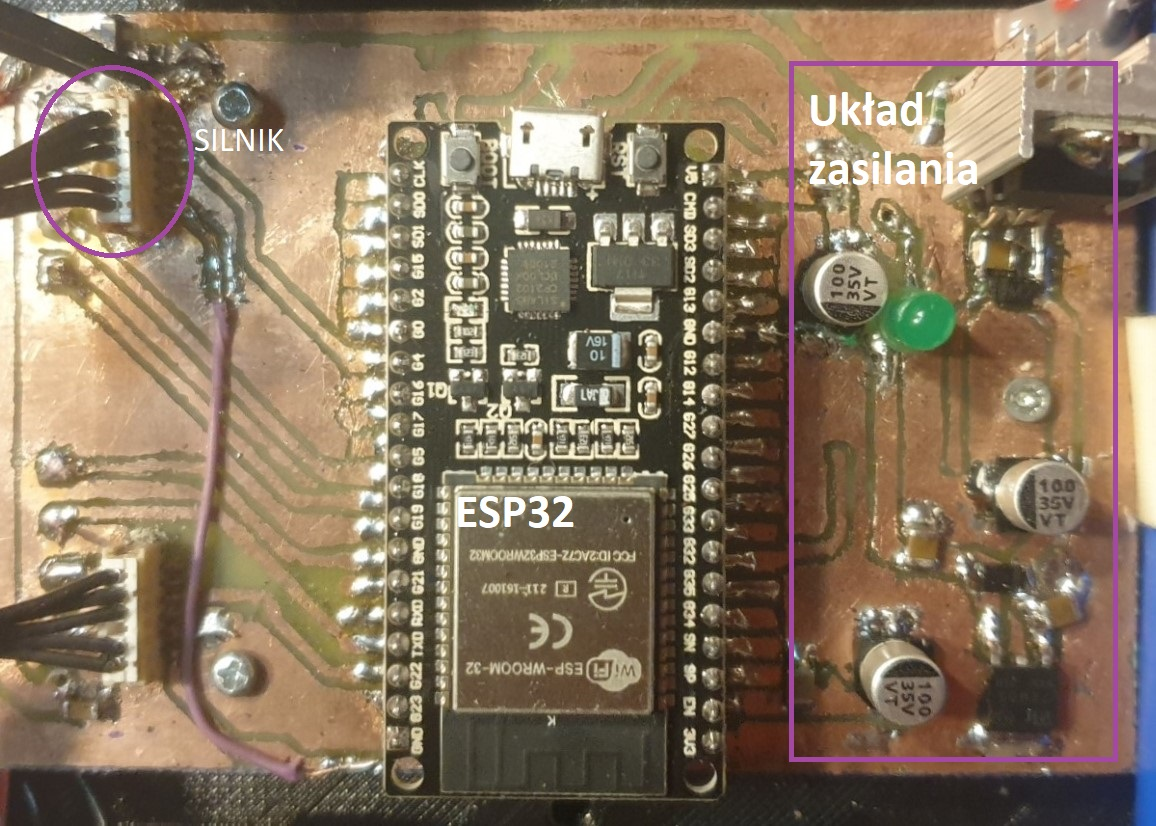
\includegraphics[width=10cm]{pages/robot/zdjecia/wykonanePCB.jpg}
	\caption{Wykonana płytka}
	\label{Fig:wykonanePCB}
\end{figure}

Płytka została wykonana na jednostronnym laminacie poprzez naniesienie utwardzalnej światłem UV maski. Pozostała nie utwardzona część maski 
została zmyta w roztworze węglanu sodu. Tak przygotowana płytka została utwardzona w 40\% roztworze chlorku żelaza(|||). 
Połączenia na dolnej warstwie zostały wykonane przy pomocy dodatkowych kabli. 

\begin{figure}[H]
	\centering
	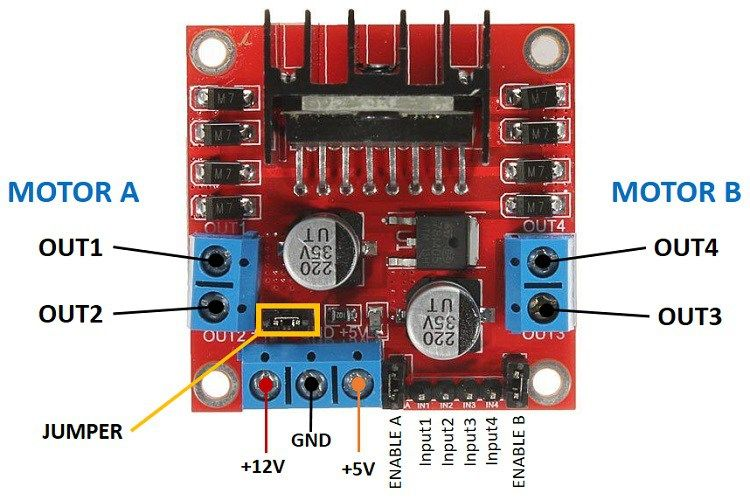
\includegraphics[width=10cm]{pages/robot/zdjecia/l298n_modul.jpg}
	\caption{Wykorzystany moduł do sterowania silnikami}
	\label{Fig:modulL298}
\end{figure}

Wykonana płytka połączona jest z zewnętrznym dwukanałowym sterownikiem silników opartym na układzie L298n. 
Sterownik maksymalnie po może obsłużyć silniki do 46V i 2A na kanał. Jego duża zaleta to praca w logice 5V 
oraz zabezpieczenie przed niedozwolonymi stanami i nadmierną temperaturą. 


\subsection{Oprogramowanie robota}

Program sterujący robotem został napisany w C++. 
Szkielet aplikacji bazuje na projekcie utworzonym przez framework IDF w wersji 4.4 udostępnionym 
przez producenta użytego procesora. Po za tym użyta została biblioteka implementująca 
system czasu rzeczywistego FreeRTOS i ASIO do obsługi połączenia TCP. 
\begin{figure}[H]
	\centering
	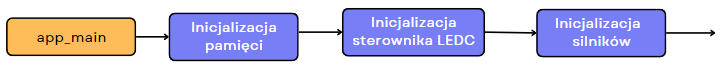
\includegraphics[width=14cm]{pages/robot/zdjecia/schematy/softSchematCz1.png}
	\caption{Schemat programu cz.1 }
	\label{Fig:Rysunek}
\end{figure}
\begin{figure}[H]
	\centering
	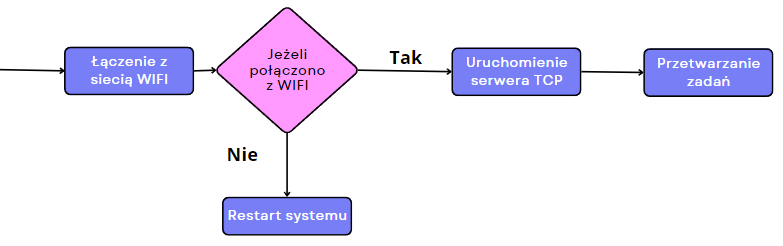
\includegraphics[width=14cm]{pages/robot/zdjecia/schematy/softSchematCz2.png}
	\caption{Schemat programu cz.2}
	\label{Fig:Rysunek}
\end{figure}

Działanie programu rozpoczyna się od wywołania funkcji app\_main, inicjalizacji funkcji systemowych i sterowników silników.
W dalszej kolejności nawiązywana jest łączność z siecią WiFi. W przypadku braku połączenia system resetuje się. 
Po poprawnym połączeniu uruchamiany jest kontekst biblioteki ASIO, a następnie uruchomienie serwera TCP.
Klienci po połączeniu do utworzonego serwera wysyłają komendy tekstowe wraz z odpowiednimi argumentami, które
robot odpowiednio przetwarza. 

\subsubsection{Sterowanie silnikami}
Sterowanie silnikami odbywa się poprzez klasę MotorController, która dziedziczy po klasie PIDController implementującej regulator PID.
Obiekt automatycznie tworzy timer uruchamiający co 100ms metodę aktualizującą wyjścia sterujące silnikiem. 
Aktualna prędkość wyznaczana jest na podstawie przerwania wyzwalanego przez enkoder silnika. Przerwanie inkrementuje licznik, 
czyszczony przez wcześniej opisany timer. Nastawy regulatora PID zostały dobrane eksperymentalnie, człon proporcjonalny wynosi 8 a całkujący i różniczkujący 0,1. 
Regulator PID możemy opisać przy pomocy wzoru:

\begin{equation}
	u(x) = e(x) * P + \int{e(x)} * I + \partial{e(x)} * D 
	\label{Eq:PID}
\end{equation}
Gdzie: $e(x)$ -- jest błędem; P,I,D -- to stałe odpowiednio członu proporcjonalnego, całkującego i różniczkującego

\begin{equation}
	e(x) = y_nast(x) - y_aktu(x)
	\label{Eq:blad}
\end{equation}
Gdzie: $y_nast(x)$ -- to nastawa regulatora, $y_aktu(x)$ -- jest rzeczywistą zmierzoną wartością
 
Powyżej przedstawiony regulator został zaimplementowany w funkcji calcOutput klasy PIDController.

\begin{lstlisting}[language=C++,caption=Zaimplementowany w C++ regulator PID,label={kodCPPPIDOutput}]
float PIDController::calcOutput(float current, float set)
{
	float error = set - current;
	float der = (error - this->_lastValue)/(_timeStep* 0.001);
	
	float output =  (this->_p * error) + 
					(this->_i * error * this->_timeStep * 0.001) + 
					(this->_d * der);

	this->_lastValue = error;
	return output;
}
\end{lstlisting}

Do wyznaczenia części różniczkującej potrzebna wartość błędu z poprzedniego wywołania pętli a ta zapisywana jest do zmiennej prywatnej klasy lastValue. 
Całkowanie zrealizowane jest poprzez pomnożenie przez krok dyskretyzacji. Stałe regulatora ustawiane są poprzez wywołanie konstruktora klasy.

Tak zaimplementowany regulator używany jest do wyznaczenia sygnału PWM, bezpośredniego sterującego układem L298n a ten silnikami. 

\begin{lstlisting}[language=C++,caption=Wyznaczenie modulacji PWM,label={kodCPPPWM}]
if(abs(setSpeed) - 1 > 0)
{
	pidToPwm = (int) this->calcOutput(abs(this->getCalculatedEngineRadialSpeed()), abs(setSpeed));
	if(setSpeed < 0)
	{
		pwmCh = 1;
	}
	else
		pwmCh = 0;

	pidToPwm += ledc_get_duty(LEDC_LOW_SPEED_MODE, this->_chanels[pwmCh]);
	pidToPwm = std::min(pidToPwm, 8192);
	pidToPwm = std::max(pidToPwm, 0);
}

// ustawienie wyjsc
ledc_set_duty(LEDC_LOW_SPEED_MODE, this->_chanels[pwmCh], (int)pidToPwm);
ledc_update_duty(LEDC_LOW_SPEED_MODE, this->_chanels[pwmCh]);

// ustawienie drugiego kanalu
ledc_set_duty(LEDC_LOW_SPEED_MODE, this->_chanels[(pwmCh==0)?1:0], 0);
ledc_update_duty(LEDC_LOW_SPEED_MODE, this->_chanels[(pwmCh==0)?1:0]);
\end{lstlisting}

W pierwszej kolejności sprawdzana jest zadana prędkość, jeżeli ta jest zbyt niska to na piny wystawiane są bezpośrednio stany niskie.
Jeżeli ustawiona prędkość jest poprawna to wyznaczamy wyjście regulatora. Sterowanie kierunkiem obrotów odbywa 
się poprzez znak zadanej prędkości a więc regulator otrzymuje wartości bezwzględne. 
Wyjście regulatora PID sumowane jest z aktualną nastawą. Wyjścia pwm skonfigurowane są w częstotliwości 5kHz i rozdzielczości 13bitów. 
Przed wysłanie nastaw do kontrolera pwm, te są obcinane do obsługiwanych zakresów (tj. 0 - 8192).

\subsubsection{Serwer TCP}

Po podłączeniu zasilania i uruchomieniu systemu robot oczekuje na polecenia wysłane do robota poprzez protokół internetowy TCP. Serwer został napisany w oparciu o bibliotekę ASIO, pozwalającą na asynchroniczną obsługę wejścia i wyjścia (w tym sieci).
\begin{figure}[H]
	\centering
	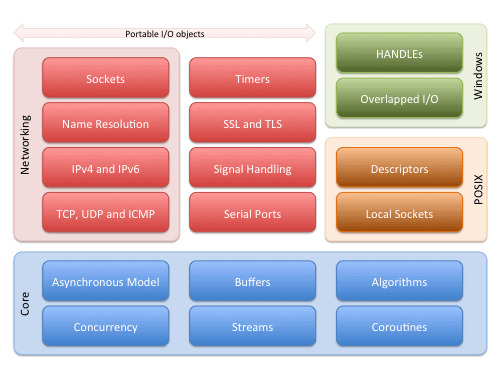
\includegraphics[width=10cm]{pages/robot/zdjecia/schematy/schematASIO.jpg}
	\caption{Schemat biblioteki ASIO \cite{asio}}
	\label{Fig:schematASIO}
\end{figure}
Biblioteka została napisana w C++ i pracuje w oparciu o standard POSIX wspierany również przez wykorzystywane ESP32.
Do akceptacji przychodzących połączeń została napisana klasa Server. Konstruktor przyjmuję referencje do kontekstu utworzonego w funkcji głównej programu. 
Uruchomienie kontekstu jest ważną częścią biblioteki ASIO, przetwarzane są w niej wszystkie asynchroniczne operacje.
Aby zapewnić jak najlepszy czas przetwarzania, kontekst uruchomiony jest w oddzielnym wątku przyłączonym do drugiego fizycznego rdzenia.

\begin{figure}[H]
	\centering
	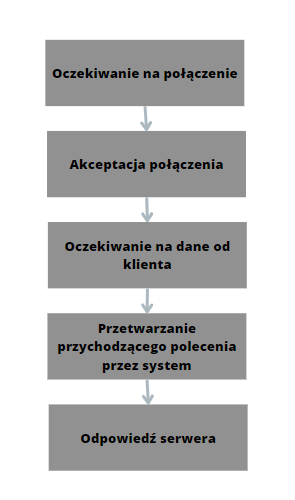
\includegraphics[width=6cm]{pages/robot/zdjecia/schematy/schematTCP.png}
	\caption{Schemat działania serwera TCP}
	\label{Fig:schematSerweraTCP}
\end{figure}

Po zaakceptowaniu przychodzącego połączenia, obiekt połączenia dodawany jest do specjalnej tablicy przechowującej wszystkich klientów. 
Dane mogą być równocześnie przetwarzane w kilku miejscach a więc używane są dzielone wskaźniki, które automatycznie usuwają dane jeżeli nikt z nich nie korzysta.
Na każdym aktywnym połączeniu prowadzony jest nasłuch, dzięki czemu możemy mieć równocześnie podłączony program do generowania ścieżki i drugi pozwalający na podgląd parametrów robota.
Klient wysyła polecenia w formie tekstowej, te przekazywane są do klasy systemowej odpowiednio interpretujące ich przeznaczenie.
Jeżeli komenda tego wymaga (np. zwrócenie prędkości obrotowej silników) to dane są odsyłane do klienta w postaci tekstu i oddzielonych przerwą liczb. 

Należy pamiętać że podczas testowania i łączenia z różnymi sieciami, serwer dhcp będzie przydzielał różne adresy ip i należy to uwzględnić w programie łączącym się z robotem.
